\chapter[Metodologia]{Metodologia}

Este capítulo descreve a metodologia proposta para o desenvolvimento deste trabalho. São inicialmente apresentadas o \textcolor{blue}{Fluxo do Metodológico} e os \textcolor{blue}{Materiais} adotados.  

\section{Fluxograma Metodológico}

De forma resumida, pretende-se seguir o seguinte fluxo de trabalho conforme mostrado na Figura \ref{fig:Fluxo}.

\begin{figure}[!htpb]
\caption{Fluxograma Metodológico}
\begin{center}
\usetikzlibrary{shapes.geometric, arrows}
\tikzstyle{startstop} = [rectangle, rounded corners, minimum width=2cm, minimum height=1cm,text centered, draw=black, fill=gray!30]
\tikzstyle{process} = [rectangle, minimum width=2cm, minimum height=1cm, text centered, draw=black, fill=white!30]
\tikzstyle{decision} = [diamond, minimum width=2cm, minimum height=1cm, text centered, draw=black, fill=yellow!30]
\tikzstyle{arrow} = [thick,->,>=stealth]

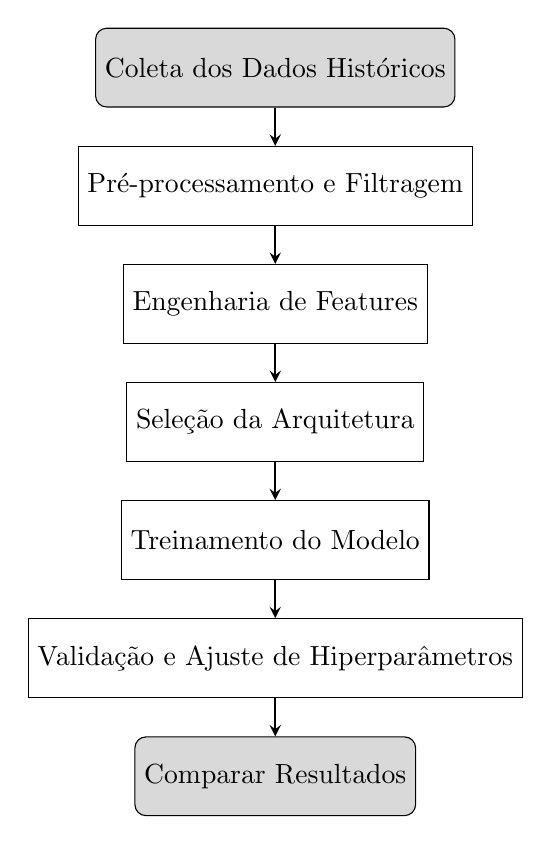
\begin{tikzpicture}[node distance=1.5cm]

    % Nodes
    % \node (start) [startstop] {Caracterização do Problema};
    \node (start) [startstop] {Coleta dos Dados Históricos};
    \node (chooseAlgo) [process, below of=start] {Pré-processamento e Filtragem};
    \node (modeling) [process, below of=chooseAlgo] {Engenharia de Features};
    \node (training) [process, below of=modeling] {Seleção da Arquitetura};
    \node (evaluation) [process, below of=training] {Treinamento do Modelo};
    \node (implementation) [process, below of=evaluation] {Validação e Ajuste de Hiperparâmetros};
    \node (deploy) [startstop, below of=implementation] {Comparar Resultados};

    % Arrows
    \draw [arrow] (start) -- (chooseAlgo);
    %\draw [arrow] (preprocess) -- (chooseAlgo);
    \draw [arrow] (chooseAlgo) -- (modeling);
    \draw [arrow] (modeling) -- (training);
    \draw [arrow] (training) -- (evaluation);
    \draw [arrow] (evaluation) -- (implementation);
    \draw [arrow] (implementation) -- (deploy);
\end{tikzpicture}
\end{center}
\fonte{Autor}
\label{fig:Fluxo}
\end{figure}


\section{Coleta de Dados Históricos} 


Os dados utilizados são provenientes do repositório oficial da RoboCup, que armazena logs públicos de partidas da SSL-B em arquivos compactados (.gz). Cada um desses logs contém informações detalhadas sobre as posições dos robôs, estado da bola, decisões do juiz e contexto do jogo. Para extração e conversão dos dados em formatos tabulares (CSV), utiliza-se a ferramenta \textit{ssl-go-tools}, que permite acessar e estruturar as informações de forma adequada para análise. Foram coletados 370.486 mil dados de treino. A estrutura dos dados já processados segue o seguinte formato:

\begin{table}[h!]
\centering
\caption{Descrição dos tipos de dados coletados na extração de logs.}
\begin{tabular}{c | c c}
\hline
\textbf{Tipo de Dado} & \textbf{Descrição} & Unidade\\
\hline
Timestamp & Marca temporal da coleta de dados & s\\
Pixel X & Posição horizontal do robô & pixels \\
Pixel Y & Posição vertical do robô em & pixels \\
X & Posição do robô no campo (coordenada X) & mm \\
Y & Posição do robô no campo (coordenada Y) & mm\\
Orientação & Orientação do robô no campo  & rad\\
\hline
\end{tabular}
\fonte{Autor}
\end{table}

A imagem a seguir mostra o processamento em tempo real de uma partida simulada a partir dos dados coletados utilizando um simulador.

\begin{figure}[!htpb]
    \centering
    \caption{Simulação de Partida com os Dados Coletados}
    \label{partida_ssl_log_player}
    \includegraphics[width=0.8\linewidth]{figuras/partida_ssl.png}
    \fonte{Autor}  
\end{figure}



\section{Pré-processamento e Filtragem} 

Na etapa de pré-processamento, pretende-se aplicar um Filtro de Kalman para criar trajetórias contínuas da bola e dos robôs, visto que os dados são obtidos de forma discreta. Feito isso, os dados serão então normalizados para o intervalo \([-1, 1]\), filtram-se registros irrelevantes para manter apenas sequências de ação contínua.  


\section{Engenharia de \textit{Features}} 

Os parâmetros de entrada do modelo representados pelas coordenadas de posição \( x(t) \) e \( y(t) \), o tempo \( t \) e a orientação angular \( \theta(t) \), além das velocidades linear e angular dos robôs. A velocidade linear \( v \) é obtida a partir das derivadas temporais da posição, enquanto a velocidade angular \( \omega \) é derivada da variação da orientação ao longo do tempo. As equações são dadas por:

\begin{equation}
    v_x(t) = \frac{dx}{dt}, \quad v_y(t) = \frac{dy}{dt}
\end{equation}

\begin{equation}
    v(t) = \sqrt{v_x^2(t) + v_y^2(t)}
\end{equation}

\begin{equation}
    \omega(t) = \frac{d\theta}{dt}
\end{equation}

onde \( v_x(t) \) e \( v_y(t) \) representam as componentes da velocidade linear nos eixos cartesianos, e \( \omega(t) \) é a velocidade angular do robô.  
  


\section{Seleção da Arquitetura}

A seleção de arquiteturas seguirá uma abordagem hierárquica, iniciando com modelos lineares clássicos como \textit{baseline} e evoluindo para arquiteturas profundas especializadas em dados sequenciais. A progressão considerou um modelo inicial para estabelecer desempenho mínimo esperado. Em seguinda, pretende-se fazer o uso das redes Recorrentes (LSTM/GRU), a escolha justifica-se pela natureza temporal dos dados e necessidade de balancear complexidade computacional com precisão preditiva.  


\section{Treinamento do Modelo}
O treinamento será realizado no \textit{framework} \textit{PyTorch}, com aceleração em GPU via CUDA. Os dados são divididos em conjuntos de treinamento selecionados de forma aleatória sendo para treinamento (70\%), validação (15\%) e teste (15\%), com \textit{early stopping} para evitar \textit{overfitting}.  

\subsection{Validação e Ajuste de Hiperparâmetros}
O modelo é avaliado por métricas como Erro Absoluto Médio (MAE) e Erro Quadrático Médio Raiz (RMSE). Uma busca em grade (grid search) otimiza hiperparâmetros críticos, como taxa de aprendizado e profundidade da rede.  



\subsection{Comparação de Resultados}  
Os resultados são comparados com algoritmos clássicos, como regressão linear e filtro de partículas, que servem como \textit{baseline}. O critério de sucesso inclui superioridade em RMSE e eficiência computacional.


\section{Materiais}


\subsection{Jupyter Notebook} O Jupyter Notebook é um ambiente interativo de código aberto para criação e compartilhamento de documentos que combinam código executável (e.g., Python, R), visualizações de dados, texto explicativo e equações. Sua estrutura baseada em células facilita a exploração iterativa de dados, prototipagem de algoritmos e documentação de fluxos de trabalho científicos.

\subsection{PyTorch} O PyTorch é uma biblioteca de aprendizado profundo baseada em tensores, destacando-se pela flexibilidade e grafos computacionais dinâmicos. Desenvolvido pelo Facebook AI Research (FAIR), permite a construção e treinamento de redes neurais, com suporte a aceleração de cálculos por GPU/TPU.

\subsection{Scipy, Matplotlib e Pandas} O Scipy oferece módulos para álgebra linear, otimização e processamento de sinais. O Matplotlib é utilizado para visualização de dados 2D/3D, enquanto o Pandas proporciona estruturas de dados eficientes para manipulação de dados tabulares, integrando-se a fluxos de trabalho de análise e machine learning.

\subsection{SSL-GO-TOOLS} O ssl-go-tool é um conjunto de pacotes em Go que facilita tarefas na RoboCup Small Size League (SSL). Oferece funcionalidades para leitura, escrita, envio, recebimento e análise de mensagens do SSL-Vision e SSL-GameController, sendo utilizado também para extrair dados de logs de partidas e rodar partidas anteriores através de um log player.